\documentclass[11pt,t]{beamer}
\usetheme{metropolis}
\metroset{progressbar=frametitle,numbering=fraction}
\setbeamertemplate{frame numbering}{\insertframenumber/\insertmainframenumber} % the total leaves out the backup after \appendix
\usefonttheme[onlymath]{serif} % serif math: proper primes, hats and italics
\usepackage{bm}
\usepackage{amsmath,amssymb,amsfonts}
\usepackage{mathrsfs}
\usepackage{booktabs}
\usepackage{multirow}
\usepackage{graphicx}
\usepackage{xcolor}
\usepackage{tikz}
\usetikzlibrary{calc,positioning,decorations.pathmorphing,decorations.fractals,decorations.markings,arrows.meta}
\setbeamercolor{block title}{use=normal text, fg=normal text.fg,bg=normal text.bg!80!fg}
\graphicspath{{./figures/}{../ModelB/Slides/figures/}{../ModelB/Slides/logo/}}

%%%%%%%%%%%%% Macros %%%%%%%%%%%%%
\newcommand{\rmi}{\mathrm{i}}
\newcommand{\rmd}{\mathrm{d}}
\newcommand{\DM}{\mathrm{DM}}

\title{Quantum Field Theory\\ meets Machine Learning}
\subtitle{}

\date{October 23, 2026}
\author{Yang-yang Tan}
\titlegraphic{%
  \begin{tikzpicture}[remember picture, overlay]
    % Top-left: occasion
    \node[anchor=north west, inner sep=0pt, font=\normalsize\bfseries, text=burgundy]
      at ([xshift=0.6cm,yshift=-0.5cm]current page.north west)
      {AI as Science Team, RIKEN iTHEMS};
    % Bottom-right: UTokyo + IPI level with the author name, so the affiliation line stays clear of the ginkgo
    \node[anchor=south east, inner sep=0pt] (utokyo) at ([xshift=-0.6cm,yshift=4.3cm]current page.south east) {%
      \raisebox{-0.5\height}{\includegraphics[height=3em]{UTokyo_Logotype_A_Color_RGB20240401.png}}%
      \hspace{0.4em}\rule[-0.9em]{0.4pt}{2em}\hspace{0.4em}%
      \raisebox{-0.5\height}{\includegraphics[height=2.3em]{ipilogo.png}}%
    };
    % Below UTokyo/IPI: RIKEN + iTHEMS (no separator)
    \node[anchor=north east, inner sep=0pt] at ([yshift=-0.5em]utokyo.south east) {%
      \raisebox{-0.5\height}{\includegraphics[height=2em]{logo_riken.pdf}}%
      \hspace{0.6em}%
      \raisebox{-0.5\height}{\includegraphics[height=2em]{logo_dark.pdf}}%
    };
  \end{tikzpicture}%
}

\definecolor{burgundy}{RGB}{127, 0, 32}
\definecolor{Kleinblue}{RGB}{0, 47, 167}
% Fira has no kana or kanji, needed for the Japanese title of the JHPCN project
\newfontfamily\jafont{Droid Sans Japanese}
% line colours of experiment_endmatter.pdf, so the legend and table match the plotted curves
\definecolor{dmline}{RGB}{0, 114, 178}
\definecolor{lvline}{RGB}{213, 94, 0}
% one colour per research direction in the plan
\colorlet{cA}{Kleinblue}
\colorlet{cB}{burgundy}
\colorlet{cC}{orange!75!black}
\newcommand{\running}[1]{\textcolor{burgundy}{#1}}
\newcommand{\kb}[1]{{\bfseries\color{Kleinblue} #1}}
% references pinned to the bottom of the page, independent of the frame content
\makeatletter
\newcommand{\refs}[1]{%
  \begin{tikzpicture}[remember picture, overlay]
    \node[anchor=south west, inner sep=0pt, align=flush left,
          text width=\dimexpr\textwidth-1.4cm\relax]
      at ([xshift=\beamer@leftmargin, yshift=0.6cm]current page.south west)
      {\raggedright\tiny\color{black!65} #1\par};
  \end{tikzpicture}}
\makeatother
\newcommand{\rtag}[1]{\textcolor{burgundy}{\textbf{#1}}}
% venue tag in the top right corner as overlay, so it costs no height
\newcommand{\venue}[1]{\begin{tikzpicture}[remember picture, overlay]
  \node[anchor=north east, font=\tiny, text=black!55] at ([xshift=-0.6cm,yshift=-1.12cm]current page.north east) {#1};
\end{tikzpicture}}

\tikzset{
  stage/.style={
    rectangle, rounded corners=3pt,
    draw=#1!80, fill=#1!12, line width=0.8pt,
    minimum width=2.8cm, minimum height=1.7cm,
    align=center, font=\small\bfseries, text=#1!50!black,
    inner sep=4pt
  },
  tlarrow/.style={
    ->, >=stealth, line width=1.4pt, draw=gray!55,
    shorten >=2pt, shorten <=2pt
  },
  % parametrized styles live outside the frames, where #1 survives
  cv/.style={anchor=north west, align=left, font=\small, inner sep=0pt},
  thread/.style={
    rectangle, rounded corners=3pt, draw=#1!70, fill=#1!5, line width=0.8pt,
    inner sep=3.5pt, align=left, font=\small
  }
}

\begin{document}
\begin{frame}[plain,noframenumbering,t]
  \inserttitlegraphic\par
  \vspace*{0.5cm}
  {\LARGE\bfseries \inserttitle\par}
  \vspace{0.4em}
  {\color{orange}\rule{\textwidth}{0.4pt}\par}
  \vspace{1.4em}
  {\normalsize\bfseries \insertauthor\par}
  \vspace{0.6em}
  {\small IPI, The University of Tokyo\par}
  \vspace{0.2em}
  {\small Long-term visitor, RIKEN iTHEMS\par}
  \vspace{0.6em}
  {\normalsize \insertdate\par}
\end{frame}

% ---------------------------------------------------------------- 1
\begin{frame}{From quantum field theory to machine learning}
  \begin{columns}[T,onlytextwidth]
    \begin{column}{0.35\textwidth}
      % inside a column \linewidth is the column width; positioning keys like below= would reset the anchor, so explicit offsets
      
\begin{tikzpicture}[every node/.append style={text width=\linewidth-4mm}]
        \node[cv] (e1) at (4mm,0) {\kb{2019--2025}\\ Ph.D.\\ Dalian Univ.\ of Tech.\\ {\footnotesize\color{black!60}advisor Wei-jie Fu}};
        \node[cv] (e2) at ([yshift=-4mm]e1.south west) {\kb{2025--2026}\\ Visitor, Tsinghua Univ.};
        \node[cv] (e3) at ([yshift=-4mm]e2.south west) {\kb{since 2026}\\ Postdoc, IPI, UTokyo\\ {\footnotesize\color{black!60}long-term visitor\\ RIKEN iTHEMS}};
        \draw[line width=1.2pt, gray!35] (0,-1mm) -- (0,0 |- e3.south);
        \foreach \e in {e1,e2,e3} \fill[Kleinblue] (0,0 |- \e.north) ++(0,-1.7mm) circle (1.1mm);
      \end{tikzpicture}
    \end{column}
    \begin{column}{0.62\textwidth}
      % venue and year in tiny, so that each item keeps one line in a box of this width
      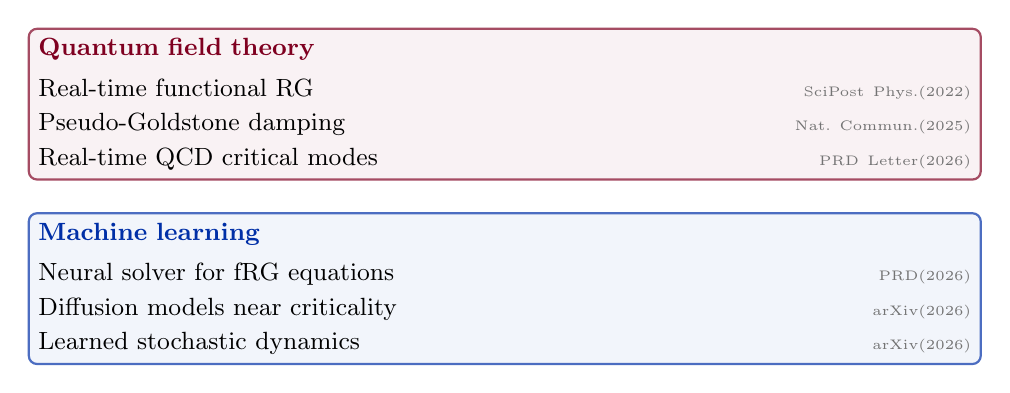
\begin{tikzpicture}[every node/.append style={text width=\linewidth-8pt}]
        \node[thread=burgundy, anchor=north] (qft) at (0,0) {%
          {\bfseries\color{burgundy}Quantum field theory}\\[0.4em]
          Real-time functional RG\hfill{\tiny\color{black!55}SciPost Phys.(2022)}\\[0.15em]
          Pseudo-Goldstone damping\hfill{\tiny\color{black!55}Nat.\ Commun.(2025)}\\[0.15em]
          Real-time QCD critical modes\hfill{\tiny\color{black!55}PRD Letter(2026)}};
        \node[thread=Kleinblue, below=4mm of qft] (ml) {%
          {\bfseries\color{Kleinblue}Machine learning}\\[0.4em]
          Neural solver for fRG equations\hfill{\tiny\color{black!55}PRD(2026)}\\[0.15em]
          Diffusion models near criticality\hfill{\tiny\color{black!55}arXiv(2026)}\\[0.15em]
          Learned stochastic dynamics\hfill{\tiny\color{black!55}arXiv(2026)}};
      \end{tikzpicture}
    \end{column}
  \end{columns}
  \vfill
  {\centering
  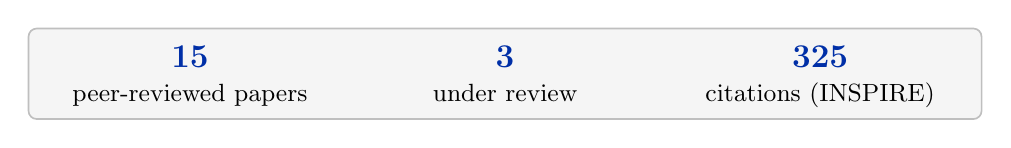
\begin{tikzpicture}
    % numbers and labels sit on fixed baselines inside the bar
    \node[rectangle, rounded corners=3pt, draw=black!25, fill=black!4, line width=0.6pt,
      minimum width=\textwidth-0.6pt, minimum height=11.5mm] (bar) {};
    \foreach \dx/\n/\l in {-0.33/15/peer-reviewed papers, 0/3/under review, 0.33/325/citations (INSPIRE)} {
      \node[anchor=base, font=\large\bfseries, text=Kleinblue] at ([xshift=\dx\textwidth,yshift=-5mm]bar.north) {\n};
      \node[anchor=base, font=\small] at ([xshift=\dx\textwidth,yshift=2.3mm]bar.south) {\l};
    }
  \end{tikzpicture}\par}
  \vspace{0.6em}
\end{frame}

\section{Critical phenomena from non-perturbative quantum field theory}

% ---------------------------------------------------------------- 2
\begin{frame}{Critical points look alike across physics}
  \begin{columns}[T,onlytextwidth]
    \begin{column}{0.32\textwidth}
      \centering
      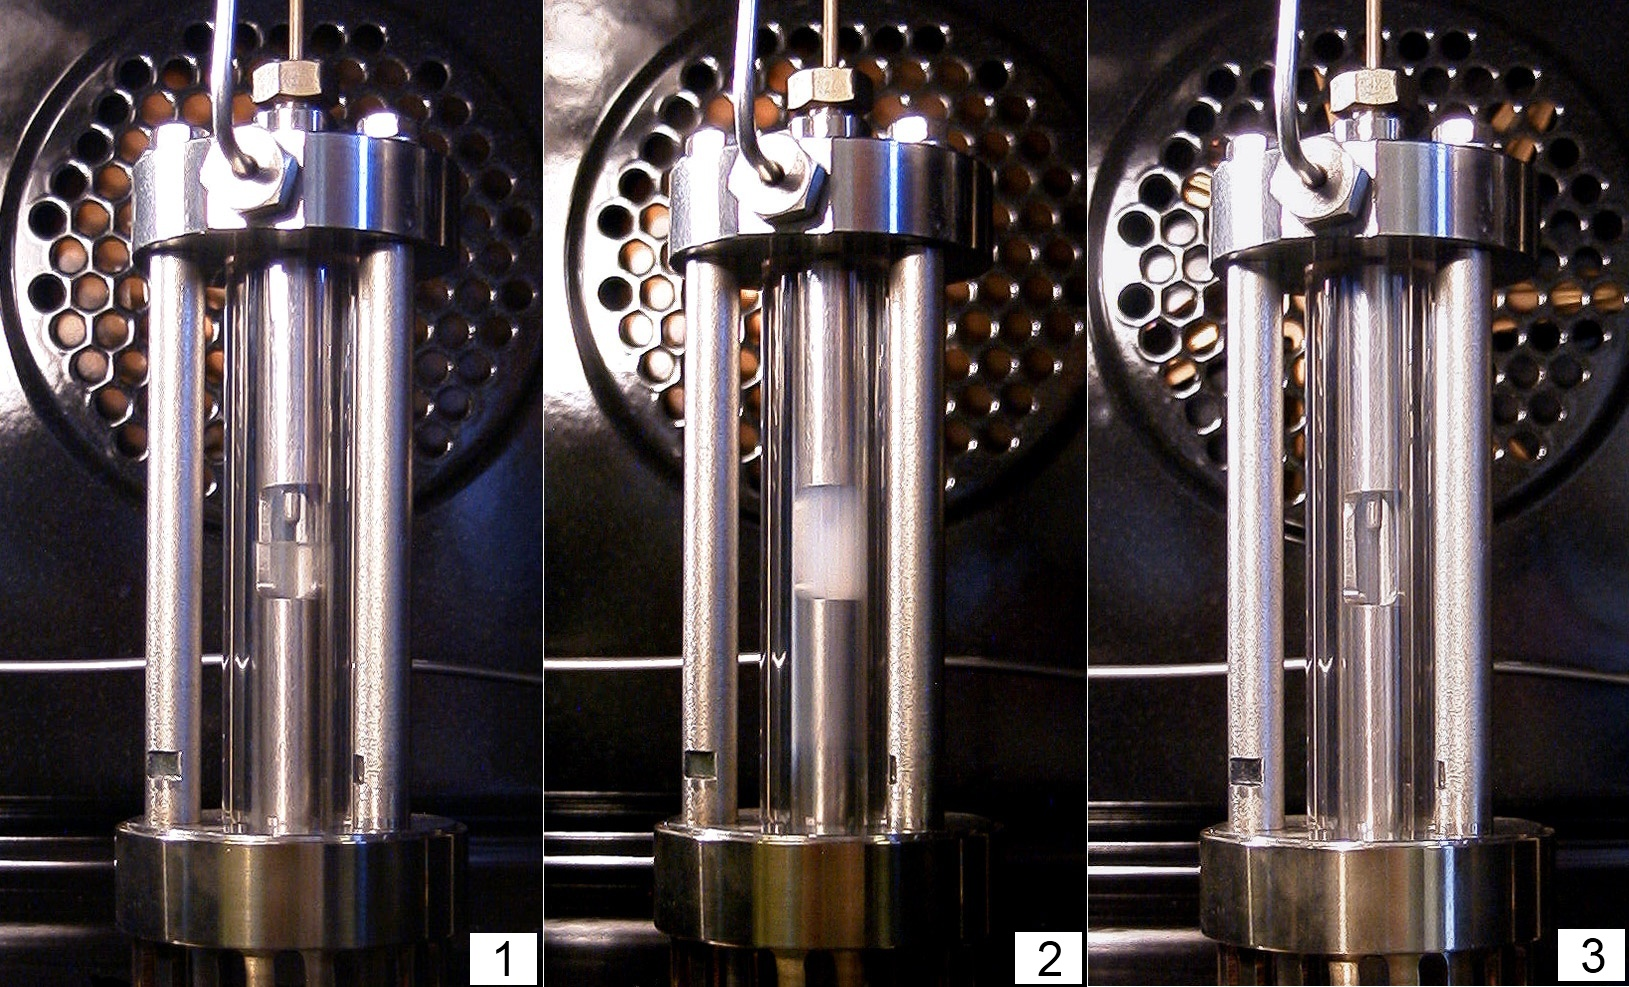
\includegraphics[height=1.6cm]{critical_opalescence_ethane.jpg}\\[0.1em]
      {\scriptsize fluids}
    \end{column}
    \begin{column}{0.32\textwidth}
      \centering
      \includegraphics[height=1.6cm]{gpmv_membrane_critical.png}\\[0.1em]
      {\scriptsize cell membranes}
    \end{column}
    \begin{column}{0.32\textwidth}
      \centering
      \includegraphics[height=1.6cm]{qcd_phase_diagram_bhalerao.png}\\[0.1em]
      {\scriptsize QCD matter}
    \end{column}
  \end{columns}
  \vspace{0.8em}
  \begin{columns}[T,onlytextwidth]
    \begin{column}{0.40\textwidth}
      \centering
      \includegraphics[width=0.78\linewidth]{coexistence_universality.pdf}\\[0.1em]
      {\scriptsize eight fluids, one curve}
    \end{column}
    \begin{column}{0.58\textwidth}
      \small\raggedright
      \kb{Universality}\\
      one set of exponents\\ for very different systems\\[0.5em]
      \kb{Non-perturbative}\\
      $\xi\to\infty$, no small parameter\\[0.5em]
      \kb{Renormalization group}\\
      systems flowing to one fixed point\\ share its exponents
    \end{column}
  \end{columns}
  \refs{%
    \rtag{Ethane} Horstmann, Wikimedia Commons.\quad
    \rtag{Membranes} Gray et al., Biophys.\ J.\ 105, 2751 (2013).\quad
    \rtag{QCD} Bhalerao, CERN-2014-001.\quad
    \rtag{Fluids} Guggenheim, J.\ Chem.\ Phys.\ 13, 253 (1945).}
\end{frame}

% ---------------------------------------------------------------- 3
\begin{frame}{The functional renormalization group for critical phenomena}
  \centering
  % Gamma_k keeps every degree of freedom down to k=0, so each panel has the same 128^2 sites and only the spacing grows as k decreases.
  % rg_zoom_b<b>.png is the central (128b)^2 window of the configuration in 2Dphi4/trainingdata/cfgs_wolff_fahmc_k=0.27088_l=0.022_1024^2.jld2
  % (WolffFAHMC_ND.jl, hot start, 500 warmup iterations, fixed metric p^2+0.01), block averaged by b and multiplied by sigma_1/sigma_b of that
  % configuration, the field rescaling of a block step, RdBu_r on +-2.5 and 6 px per site as phi4_snapshot. The white square marks the previous panel
  \begin{tikzpicture}[x=1mm, y=1mm, lab/.style={font=\scriptsize, align=center, text=black!70}]
    \foreach \b [count=\i] in {1, 2, 4, 8}
      \node[inner sep=0pt] (z\i) at (22*\i-22,0) {\includegraphics[width=1.05cm]{rg_zoom_b\b.png}};
    % zoom lines from the corners of each panel to the corners of its region in the next one
    \foreach \i/\j in {1/2, 2/3, 3/4}
      \draw[black!45, line width=0.5pt] (z\i.north east) -- ($(z\j.center)+(-2.625,2.625)$) (z\i.south east) -- ($(z\j.center)+(-2.625,-2.625)$);
    \foreach \i in {2,3,4} \draw[white, line width=0.6pt] ($(z\i.center)+(-2.625,-2.625)$) rectangle ($(z\i.center)+(2.625,2.625)$);
    \draw[tlarrow] (z1) -- (z2); \draw[tlarrow] (z2) -- (z3); \draw[tlarrow] (z3) -- (z4);
    \node[lab, anchor=north] at (z1.south) {microscopic\\ $\Gamma_{k=\Lambda}=S$};
    \node[lab, anchor=north] at (z4.south) {all fluctuations\\ $\Gamma_{k=0}=\Gamma$};
    % what Gamma is, between its two ends S and Gamma
    \node[lab, anchor=north] at (33,-5.6) {$\Gamma[\phi]=\sup_J\big(J\!\cdot\!\phi-\ln Z[J]\big)$\\ {\tiny\color{black!55}Legendre transform of the generating functional}};
    \node[lab] at (33,8.5) {as $k$ decreases, $\Gamma_k$ takes in the fluctuations shell by shell};
  \end{tikzpicture}\par
  \vspace{-0.6em}
  {\small $k\partial_k\Gamma_k=\tfrac12\,\mathrm{Tr}\big[(\Gamma_k^{(2)}+R_k)^{-1}\,k\partial_kR_k\big]$\quad{\footnotesize\color{black!60} exact RG}\par}
  \vspace{0em}
  \begin{columns}[T,onlytextwidth]
    \begin{column}{0.48\textwidth}
      \centering
      \kb{Critical point}\\[0.2em]
      % after Fig. 23 of Tong's Statistical Field Theory notes, laid on its side. The sheet is the critical surface, dashed blue arrows are
      % irrelevant flows into the fixed point, the burgundy arrow is the relevant direction, the two black curves start near the surface,
      % come close to the fixed point and leave along the relevant direction
      % both diagrams in boxes of one height, so the two captions below share a baseline
      \parbox[c][22mm][c]{\linewidth}{\centering
      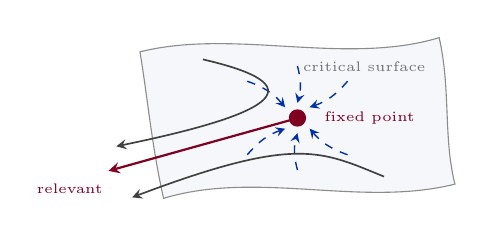
\begin{tikzpicture}[x=1mm, y=1.2mm, >=stealth, lab/.style={font=\tiny, text=black!55}]
        \filldraw[fill=cA!4, draw=black!45, line width=0.4pt]
          (-20,7) .. controls (-8,9.5) and (6,5.5) .. (18,8.5) .. controls (19.5,3) and (18.5,-2) .. (20,-7)
          .. controls (8,-9.5) and (-5,-5.5) .. (-17,-8.5) .. controls (-18.5,-3) and (-19,2) .. cycle;
        % no irrelevant arrow at 0 and 180 degrees, where the label and the relevant direction sit
        \foreach \t in {45, 90, 135, 225, 270, 315}
          \draw[->, cA, dashed, line width=0.5pt] ({9*cos(\t)},{5.5*sin(\t)}) to[bend left=15] ({2.2*cos(\t)},{1.6*sin(\t)});
        \draw[->, black!75, line width=0.6pt] (-12,6.2) .. controls (2,3.5) and (-2,0.6) .. (-23,-3.0);
        \draw[->, black!75, line width=0.6pt] (11,-6.2) .. controls (3,-3.5) and (0,-1.8) .. (-21,-8.4);
        \draw[->, cB, line width=0.8pt] (-1,-0.25) -- (-24,-5.6);
        % radius in mm, so the y stretch of the picture keeps the dot round
        \fill[cB] (0,0) circle (1.1mm);
        \node[lab, anchor=north east] at (17.5,7.0) {critical surface};
        \node[lab, text=cB, anchor=west] at (2.2,0) {fixed point};
        \node[lab, text=cB, anchor=north east] at (-23.5,-5.9) {relevant};
      \end{tikzpicture}}\\[0.7em]
      {\footnotesize global fixed point\par}
      \vspace{0.25em}
      {\tiny\color{black!55}\textbf{Tan}, Huang, Chen, Fu, Eur.\ Phys.\ J.\ C 84, 897 (2024)\par}
    \end{column}
    \begin{column}{0.48\textwidth}
      \centering
      \kb{Real time}\\[0.2em]
      % Schwinger-Keldysh contour in the complex t plane, forward on C+ and back on C-.
      % Arrow positions are the midpoints of the two legs as fractions of the path length 22+1.2pi+22
      \parbox[c][22mm][c]{\linewidth}{\centering
      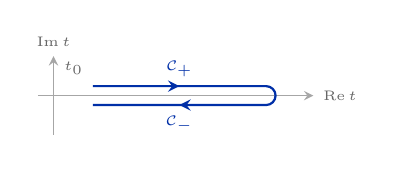
\begin{tikzpicture}[x=1mm, y=1mm, >=stealth, lab/.style={font=\tiny, text=black!60}]
        \draw[->, black!35, line width=0.5pt] (-2,0) -- (33,0) node[right, lab] {$\mathrm{Re}\,t$};
        \draw[->, black!35, line width=0.5pt] (0,-5) -- (0,5) node[above, lab] {$\mathrm{Im}\,t$};
        \draw[cA, line width=0.8pt, postaction={decorate}, decoration={markings,
            mark=at position 0.23 with {\arrow{stealth}}, mark=at position 0.77 with {\arrow{stealth}}}]
          (5,1.2) -- (27,1.2) arc (90:-90:1.2) -- (5,-1.2);
        \node[font=\tiny, text=cA] at (16,3.4) {$\mathcal{C}_+$};
        \node[font=\tiny, text=cA] at (16,-3.6) {$\mathcal{C}_-$};
        \node[lab, anchor=south east] at (5,1.4) {$t_0$};
      \end{tikzpicture}}\\[0.7em]
      {\footnotesize the same flow on the closed time path\par}
      \vspace{0.25em}
      {\tiny\color{black!55}\textbf{Tan}, Chen, Fu, SciPost Phys.\ 12, 026 (2022)\par}
      {\tiny\color{black!55}\rtag{Model A} Chen, \textbf{Tan}, Fu, PRD 109, 094044 (2024)\par}
      {\tiny\color{black!55}\rtag{Model H} Chen, \textbf{Tan}, Fu, PRD 111, 094025 (2025)\par}
    \end{column}
  \end{columns}
\end{frame}

% ---------------------------------------------------------------- 4
\begin{frame}{Criticality breaks the GMOR and damping relations}
  \small
  \kb{Pseudo-Goldstone modes near a critical point}\par
  \vspace{0.4em}
  {\centering
  \begin{tabular}{@{}lcc@{}}
    & away from $T_c$ & near $T_c$\\
    \midrule
    GMOR & $m_\varphi^2\propto m_q$ & $m_\varphi^2\propto m_q^{\,2\nu/\beta\delta}$\\[0.25em]
    damping & $\Omega_\varphi/m_\varphi^2\simeq D_\varphi$ & $\Omega_\varphi/m_\varphi^2\propto m_\varphi^{\,\eta_t-\eta}$\\
  \end{tabular}\par}
  \vspace{0.4em}
  {\centering \kb{New universal damping} set by $\eta_t-\eta$, beyond hydro and holography\par}
  \vspace{0.4em}
  \begin{columns}[T,onlytextwidth]
    \begin{column}{0.38\textwidth}
      \centering
      \includegraphics[width=0.82\linewidth]{mexican_hat_goldstone}\\[0.1em]
      {\footnotesize a slightly tilted hat\\ droplets roll\par}
    \end{column}
    \begin{column}{0.60\textwidth}
      \centering
      % pseudo-Goldstone modes across physics; x and y in mm
      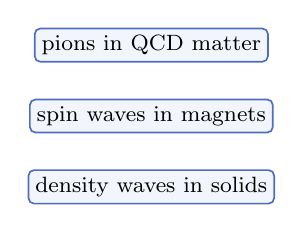
\begin{tikzpicture}[x=1mm, y=1mm,
          leaf/.style={draw=Kleinblue!70, fill=Kleinblue!5, rounded corners=2pt, line width=0.6pt,
            inner sep=2.5pt, font=\footnotesize, align=center}]
        \node[leaf] at (0,9) {pions in QCD matter};
        \node[leaf] at (0,0) {spin waves in magnets};
        \node[leaf] at (0,-9) {density waves in solids};
      \end{tikzpicture}\\[0.4em]
      {\footnotesize damping fixed by the universality class alone\par}
    \end{column}
  \end{columns}
  \venue{\textbf{Tan}, Chen, Fu, Li, Nature Commun.\ 16, 2916 (2025)}
\end{frame}

% ---------------------------------------------------------------- 5
\begin{frame}{Critical slowing down in heavy-ion collisions}
  % cartoon of a collision, x and y in mm; the body must not open with a brace group, which beamer would take as a subtitle
  % the cartoon starts below the citation in the top right corner
  \centering
  \vspace{0.7em}
  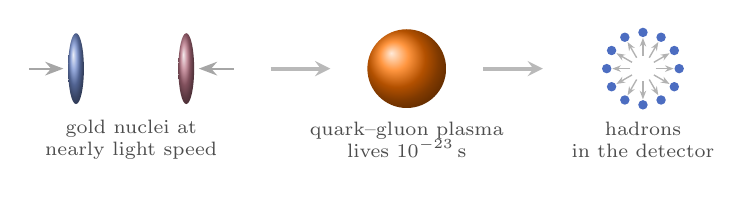
\begin{tikzpicture}[x=1mm, y=1mm, lab/.style={font=\scriptsize, align=center, text=black!70}]
    \shade[ball color=Kleinblue!55] (0,0) ellipse (1 and 4.5);
    \shade[ball color=burgundy!55] (14,0) ellipse (1 and 4.5);
    \draw[-{Stealth}, line width=0.8pt, gray!70] (-6,0) -- (-1.6,0);
    \draw[-{Stealth}, line width=0.8pt, gray!70] (20,0) -- (15.6,0);
    \node[lab] at (7,-9) {gold nuclei at\\ nearly light speed};
    \draw[tlarrow] (24,0) -- (33,0);
    \shade[ball color=orange!90!red] (42,0) circle (5);
    \node[lab] at (42,-9) {quark--gluon plasma\\ lives $10^{-23}$\,s};
    \draw[tlarrow] (51,0) -- (60,0);
    \foreach \a in {0,30,...,330} {
      \draw[-{Stealth[length=1.1mm]}, line width=0.5pt, gray!60] ($(72,0)+(\a:1.6)$) -- ($(72,0)+(\a:3.9)$);
      \fill[Kleinblue!70] ($(72,0)+(\a:4.6)$) circle (0.6);
    }
    \node[lab] at (72,-9) {hadrons\\ in the detector};
  \end{tikzpicture}\par
  \vspace{0.3em}
  \begin{columns}[T,onlytextwidth]
    \begin{column}{0.48\textwidth}
      \centering
      % image coordinates run from 0 to 1 across the picture, the arrow is the cooling fireball
      \begin{tikzpicture}
        \node[anchor=south west, inner sep=0] (pd) at (0,0) {\includegraphics[width=0.84\linewidth]{qcd_phase_diagram_bhalerao.png}};
        \begin{scope}[x={(pd.south east)}, y={(pd.north west)}]
          \draw[-{Stealth[length=2mm]}, line width=1.6pt, orange!90!red, opacity=0.85]
            (0.47,0.84) .. controls (0.36,0.73) and (0.32,0.64) .. (0.24,0.42);
        \end{scope}
      \end{tikzpicture}\\[0.1em]
      {\footnotesize path of the cooling fireball\par}
    \end{column}
    \begin{column}{0.50\textwidth}
      \centering
      \includegraphics[width=0.8\linewidth]{qcd_relaxation_time_3d}\\[0.1em]
      {\footnotesize slow only near the critical point\par}
      {\scriptsize from QCD, \kb{no free parameters}\par}
    \end{column}
  \end{columns}
  \venue{\textbf{Tan}, Yin, Chen, Huang, Fu, Phys.\ Rev.\ D 114, L011501 (2026)}
  \refs{%
    Phase diagram after Bhalerao.}
\end{frame}

\section{Machine learning for non-perturbative field theory}

% ---------------------------------------------------------------- 6
\begin{frame}{Large $N$ absorbs the stiffness, a network learns the rest}
  \begin{columns}[T,onlytextwidth]
    \begin{column}{0.44\textwidth}
      \centering
      \kb{Fluctuations flatten $V_k$}\\[0.6em]
      % cartoon of convexity restoration, a double well flattens between its minima as k goes to 0.
      % Colours follow the paper, UV red, lower k blue, IR orange. The curves share the walls, so the lower-k ones are drawn
      % only between the minima and the UV double well stays whole
      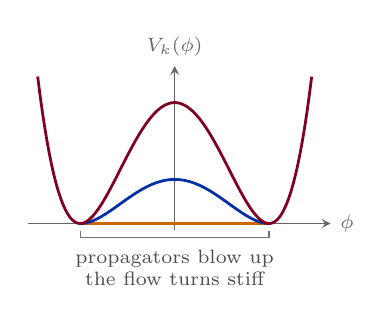
\begin{tikzpicture}[x=6mm, y=16mm]
        \draw[->, >=stealth, black!60] (-3.1,0) -- (3.3,0) node[right, font=\scriptsize] {$\phi$};
        \draw[->, >=stealth, black!60] (0,-0.05) -- (0,1.25) node[above, font=\scriptsize] {$V_k(\phi)$};
        \draw[orange!80!black, line width=1.3pt] (-2,0) -- (2,0);
        \draw[cA, line width=1pt, domain=-2:2, samples=100] plot (\x, {0.35*(1-\x*\x/4)^2});
        \draw[cB, line width=1pt, domain=-2.9:2.9, samples=120] plot (\x, {0.06*(\x*\x-4)^2});
        % on the flat bottom k^2+V_k'' goes to zero, so the regulated propagators diverge
        \draw[black!55, line width=0.5pt] (-2,-0.06) -- (-2,-0.11) -- (2,-0.11) -- (2,-0.06);
        \node[font=\scriptsize, text=black!70, anchor=north, align=center] at (0,-0.13) {propagators blow up\\ the flow turns stiff};
      \end{tikzpicture}\\[0.5em]
      {\scriptsize\textcolor{cB}{$k=\Lambda$}\quad\textcolor{cA}{lower $k$}\quad\textcolor{orange!80!black}{$k\to0$}\par}
    \end{column}
    \begin{column}{0.54\textwidth}
      \centering
      \kb{Physics does the hard part}\\[0.6em]
      % V_k' split into the exact large-N part and the learned rest, sketches only. On the flat bottom V_k'=-k^2 for any N,
      % so the rest vanishes there and sits just outside it, as the learned correction in the paper does.
      % The rest is the full curve times exp(-d^2/0.2^2), so the large-N curve keeps the flat bottom a little longer and then turns up sharper
      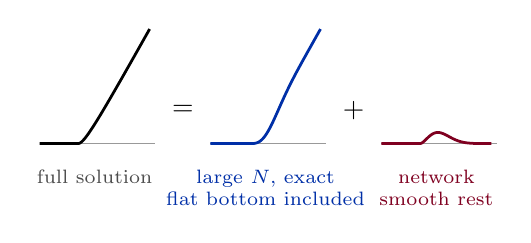
\begin{tikzpicture}[x=14mm, y=14mm, lab/.style={font=\scriptsize, align=center, text=black!70}]
        \foreach \xa in {0, 1.55, 3.1} \draw[black!40] (\xa,0) -- (\xa+1.05,0);
        \draw[black, line width=1pt, domain=0:1, samples=100] plot (\x, {1.8*max(\x-0.35,0)^2/(max(\x-0.35,0)+0.08)});
        \draw[cA, line width=1pt, domain=0:1, samples=100] plot (1.55+\x, {1.8*max(\x-0.35,0)^2/(max(\x-0.35,0)+0.08)*(1-exp(-(max(\x-0.35,0)/0.2)^2))});
        \draw[cB, line width=1pt, domain=0:1, samples=100] plot (3.1+\x, {1.8*max(\x-0.35,0)^2/(max(\x-0.35,0)+0.08)*exp(-(max(\x-0.35,0)/0.2)^2)});
        \node at (1.3,0.3) {$=$};
        \node at (2.85,0.3) {$+$};
        \node[lab, anchor=north] at (0.5,-0.15) {full solution};
        \node[lab, anchor=north, text=cA] at (2.05,-0.15) {large $N$, exact\\ flat bottom included};
        \node[lab, anchor=north, text=cB] at (3.6,-0.15) {network\\ smooth rest};
      \end{tikzpicture}\\[1.2em]
      % network of the paper. Its output is multiplied by t=ln(k/Lambda), so the correction vanishes at k=Lambda
      \includegraphics[width=\linewidth]{neural_frg_architecture}
    \end{column}
  \end{columns}
  \venue{\textbf{Tan}, Fu, He, Wang, Phys.\ Rev.\ D 114, 036026 (2026)}
\end{frame}

\section{Generative model as quantum field theory}

% ---------------------------------------------------------------- 7
\begin{frame}{A generative model is a field theory}
  \centering
  \begin{tikzpicture}[font=\scriptsize, >=stealth]
    \foreach \t/\i in {0/0,0.01/1,0.03/2,0.08/3,1/4}
      \node[inner sep=0pt] (p\i) at (1.75*\i,0) {\includegraphics[width=1.1cm]{phi4_diffuse_t\t.png}};
    \draw[->,thick,burgundy] ([yshift=0.1cm]p0.north west) -- ([yshift=0.1cm]p4.north east)
      node[midway,above] {add noise};
    \draw[<-,thick,Kleinblue] ([yshift=-0.1cm]p0.south west) -- ([yshift=-0.1cm]p4.south east)
      node[midway,below] {remove the noise with a learned force};
  \end{tikzpicture}\par
  \vspace{0.8em}
  {\small
  \begin{tabular}{@{}l@{\hspace{2.5em}}l@{}}
    \toprule
    \kb{field theory} & \kb{generative model}\\
    \midrule
    stochastic quantization & diffusion sampling\\[0.15em]
    force $-\delta S/\delta\phi$ & learned score $s_\theta(\phi,t\to0)$\\[0.15em]
    coarse-graining scale & noise level $t$\\[0.15em]
    real-time stochastic dynamics & conditional generation\\
    \bottomrule
  \end{tabular}\par}
  \refs{%
    \rtag{Stochastic quantization} Parisi, Wu, Sci.\ Sin.\ 24, 483 (1981).\quad
    \rtag{Diffusion models} Wang, Aarts, Zhou, JHEP 05, 060 (2024).\quad Hirono, Tanaka, Fukushima, arXiv:2403.11262.}
\end{frame}

% ---------------------------------------------------------------- 8
\begin{frame}{The network learns $-\delta S/\delta\phi$ from samples}
  \begin{columns}[T,onlytextwidth]
    \begin{column}{0.60\textwidth}
      \centering
      \vspace{0.3em}
      \begin{tikzpicture}[x=1mm, y=1mm,
          lab/.style={font=\scriptsize, align=center, text=black!70},
          box/.style={draw=Kleinblue!70, fill=Kleinblue!5, rounded corners=3pt, line width=0.7pt, inner sep=3.5pt, font=\small, align=center}]
        \node[inner sep=0pt] (img) at (0,0) {\includegraphics[width=1.1cm]{phi4_snapshot_k0.2705.png}};
        \node[lab, anchor=north] at (img.south) {samples of $\phi$};
        \node[box] (net) at (19,0) {network};
        \node[box] (f) at (41,0) {learned force\\ $s_\theta(\phi)$};
        \draw[tlarrow] (img.east) -- (net.west);
        \draw[tlarrow] (net.east) -- (f.west);
        \node[box, draw=burgundy!70, fill=burgundy!5] (s) at (41,-17) {true force\\ $-\delta S/\delta\phi$};
        \draw[<->, line width=1pt, gray!60] (f.south) -- node[right, lab] {compare} (s.north);
        \node[lab, text=burgundy] at (19,-17) {the action $S$\\ is never shown};
      \end{tikzpicture}
    \end{column}
    \begin{column}{0.38\textwidth}
      \centering
      \vspace{1.9em}
      {\LARGE\bfseries\color{Kleinblue}0.998\par}
      {\footnotesize alignment with the true force\par}
    \end{column}
  \end{columns}
  \vspace{0.2em}
  \kb{An exact testbed for ML algorithms/generative models}\par
  \vspace{0.3em}
  % a drawn photo icon stands for any image data set
  {\centering\footnotesize
  \renewcommand{\arraystretch}{1.1}
  \begin{tabular}{@{}l@{\hspace{2em}}c@{\hspace{2em}}c@{}}
    &
    
\begin{tikzpicture}[x=0.6mm, y=0.6mm, baseline=1.5mm]
      \draw[black!60, line width=0.5pt, rounded corners=0.6pt] (0,0) rectangle (13,10);
      \fill[black!25] (1,1) -- (4.8,6) -- (7.5,3.2) -- (9.7,5.5) -- (12,1) -- cycle;
      \fill[orange!70] (10,7.8) circle (1.1);
    \end{tikzpicture}\ images
    &
    \raisebox{-0.25\height}{\includegraphics[height=0.6cm]{phi4_snapshot_k0.2705.png}}\ lattice field theory\\
    \midrule
    distribution & {\color{black!55}unknown} & \textcolor{Kleinblue}{$e^{-S[\phi]}$, exact}\\
    structure & {\color{black!55}partly known} & \textcolor{Kleinblue}{symmetry, UV and IR known}\\
    difficulty & {\color{black!55}fixed} & \textcolor{Kleinblue}{quantitatively controllable}\\
    \bottomrule
  \end{tabular}\par}
  \vspace{0.3em}
  {\footnotesize Find which algorithm or architecture suits which structure.\par}
  \venue{\textbf{Tan}, Aarts, Habibi, Lucini, Wang, arXiv:2607.08505}
\end{frame}

% ---------------------------------------------------------------- 9
\begin{frame}{The learned theory sits at the right fixed point}
  \begin{columns}[T,onlytextwidth]
    \begin{column}{0.46\textwidth}
      \centering
      \kb{The critical exponent}\\[0.3em]
      \includegraphics[width=\linewidth]{prop_k=0.2705_log_log.pdf}\\[0.2em]
      {\small $\eta=1/4$, the exact 2D Ising value\par}
    \end{column}
    \begin{column}{0.52\textwidth}
      \centering
      \kb{Lattices never seen}\\[0.5em]
      % top left corners of one critical configuration, 6 px per site, so 8, 16 and 32 sites wide
      \begin{tikzpicture}[x=1mm, y=1mm]
        \node[inner sep=0pt] (a) at (0,9) {\includegraphics[width=0.35cm, trim=0 518.4bp 518.4bp 0, clip]{phi4_snapshot_k0.2705.png}};
        \node[inner sep=0pt] (b) at (0,1) {\includegraphics[width=0.6cm, trim=0 483.84bp 483.84bp 0, clip]{phi4_snapshot_k0.2705.png}};
        \node[inner sep=0pt] (c) at (0,-10) {\includegraphics[width=1.0cm, trim=0 414.72bp 414.72bp 0, clip]{phi4_snapshot_k0.2705.png}};
        \node[inner sep=0pt] (big) at (34,0) {\includegraphics[width=2.6cm]{phi4_snapshot_k0.2705.png}};
        \draw[tlarrow] (7,0) -- node[above, font=\scriptsize, text=black!70] {network} (big.west);
      \end{tikzpicture}\\[0.5em]
      {\small train on small lattices only\\
      generate a lattice twice as large\\
      as accurate as training on it\par}
    \end{column}
  \end{columns}
  \venue{\textbf{Tan}, Aarts, Habibi, Lucini, Wang, arXiv:2607.08505}
\end{frame}

% ---------------------------------------------------------------- 10
\begin{frame}{From statics to real-time dynamics}
  \centering
  \vspace{0.3em}
  % the two burgundy lines are the two gaps, the statics has no time and the real-time law is rarely known
  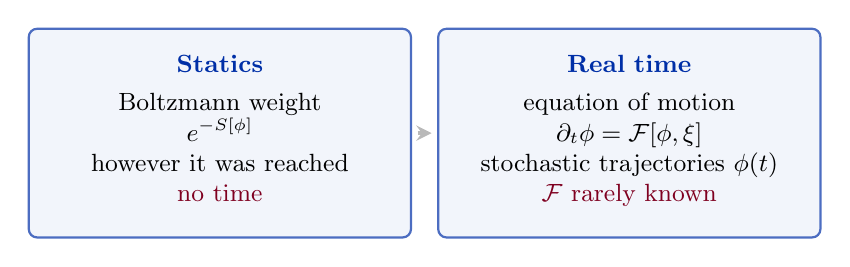
\begin{tikzpicture}[x=1mm, y=1mm, every node/.append style={minimum height=26.5mm}]
    \node[thread=cA, align=center, anchor=north, text width=0.38\textwidth] (s) at (-26,0) {%
      {\bfseries\color{cA}Statics}\\[0.3em]
      Boltzmann weight\\ $e^{-S[\phi]}\vphantom{\mathcal F[\phi,\xi]}$\\ however it was reached\\ \textcolor{burgundy}{no time}\strut};
    \node[thread=cA, align=center, anchor=north, text width=0.38\textwidth] (d) at (26,0) {%
      {\bfseries\color{cA}Real time}\\[0.3em]
      equation of motion\\ \mbox{$\partial_t\phi=\mathcal F[\phi,\xi]\vphantom{e^{-S[\phi]}}$}\\ stochastic trajectories $\phi(t)$\\ \textcolor{burgundy}{$\mathcal F$ rarely known}\strut};
    \draw[tlarrow] (s) -- (d);
  \end{tikzpicture}\par
  \vspace{0.8em}
  {\scriptsize
  \begin{tabular}{@{}c@{\hspace{6pt}}c@{\hspace{6pt}}c@{\hspace{6pt}}c@{}}
    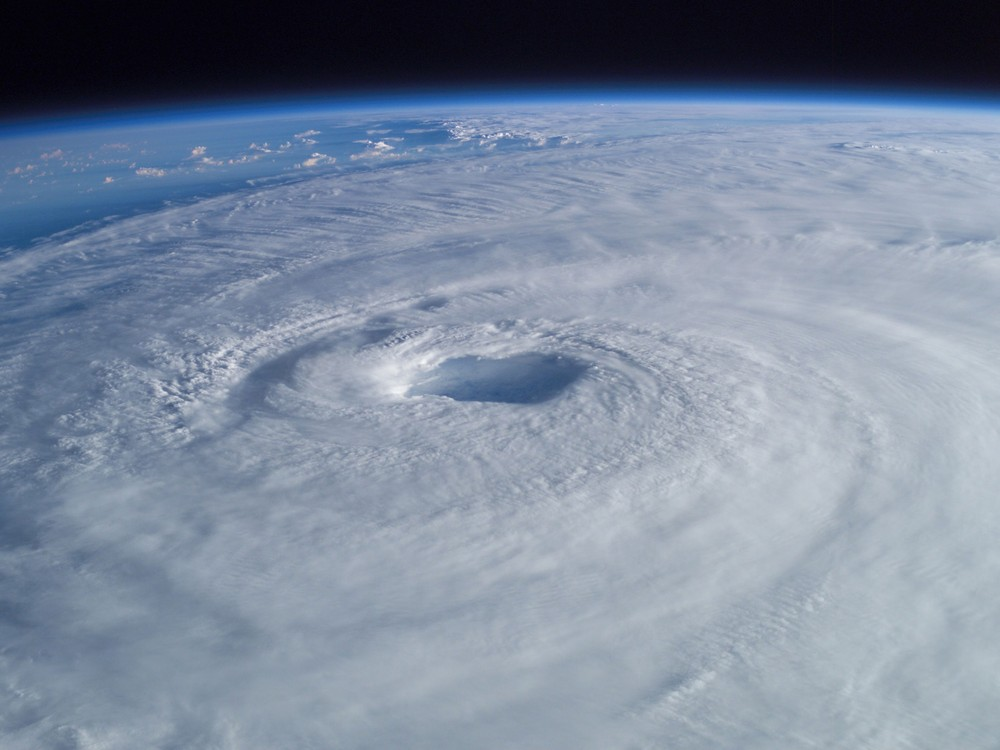
\includegraphics[height=1.45cm]{hurricane_isabel.jpg} &
    \includegraphics[height=1.45cm]{myoglobin.png} &
    \includegraphics[height=1.45cm]{colloid_tracks.png} &
    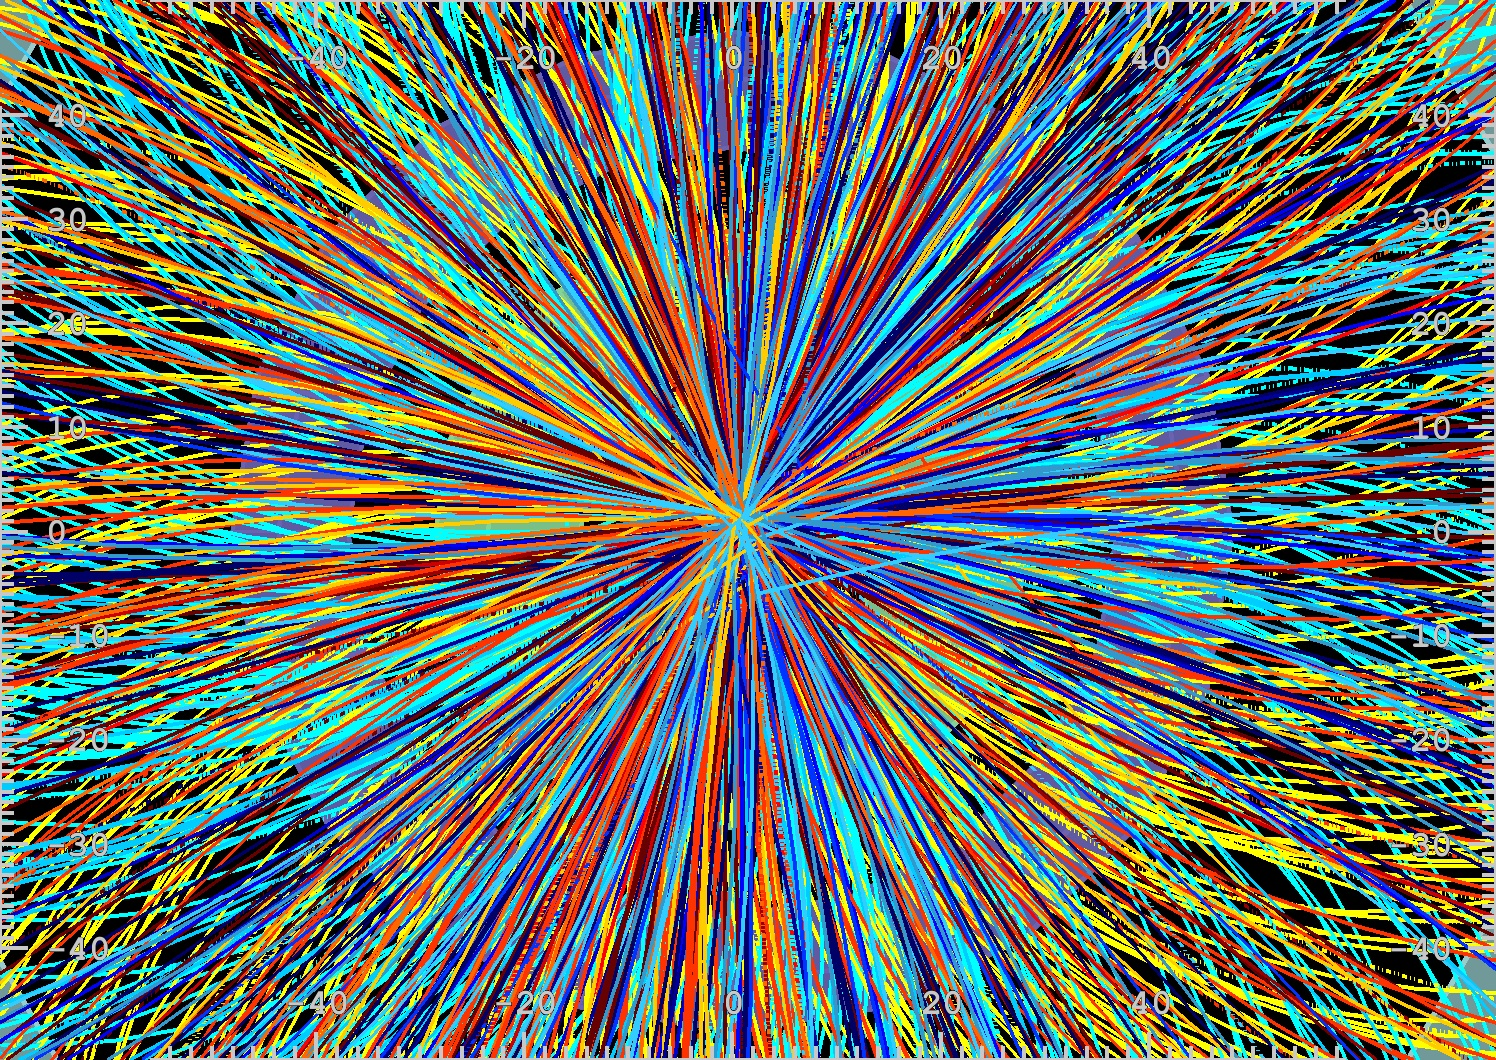
\includegraphics[height=1.45cm]{alice_pbpb_event.jpg}\\
    weather & protein dynamics & driven colloids & heavy-ion collision
  \end{tabular}\par}
  \vspace{0.8em}
  {\small\kb{Goal}\quad predict long-time dynamics from short-time data, without $\mathcal F$\par}
  \refs{%
    \rtag{Hurricane Isabel} NASA.\quad
    \rtag{Myoglobin} Wikimedia Commons.\quad
    \rtag{ALICE event display} CERN.\quad
    \rtag{Colloids} Dieball et al., Soft Matter 21, 2170 (2025).\quad
    \rtag{Learned dynamics} weather, Price et al., Nature 637, 84 (2025). Proteins, Schreiner, Winther, Olsson, NeurIPS (2023).}
\end{frame}

% ---------------------------------------------------------------- 11
\begin{frame}{Learning an effective theory in real time}
  \centering
  \vspace{0.45em}
  % the method first, then what the learned object is
  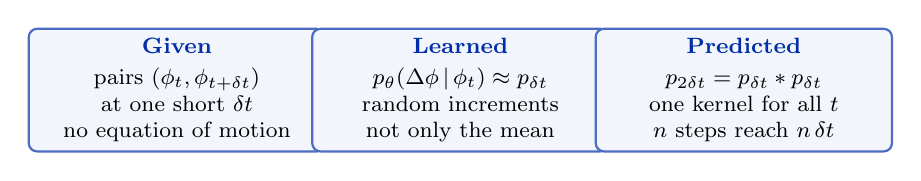
\begin{tikzpicture}[x=1mm, y=1mm]
    \foreach \x/\head/\body in {
        0/{Given}/{pairs $(\phi_t,\phi_{t+\delta t})$\\ at one short $\delta t$\\ no equation of motion},
        36/{Learned}/{\mbox{$p_\theta(\Delta\phi\,|\,\phi_t)\approx p_{\delta t}$}\\ random increments\\ not only the mean},
        72/{Predicted}/{\mbox{$p_{2\delta t}=p_{\delta t}\ast p_{\delta t}$}\\ one kernel for all $t$\\ $n$ steps reach $n\,\delta t$}}
      \node[thread=cA, align=center, anchor=north, text width=0.29\textwidth, font=\footnotesize] at (\x,0)
        {{\bfseries\color{cA}\head}\\[0.2em] \body};
  \end{tikzpicture}\par
  \vspace{0.15em}
  % Fig. 1 of the paper. Upper row the physical time, lower row one draw of the learned kernel
  \includegraphics[width=0.5\textwidth]{schematic}\par
  % delta t -> 0 leaves the equation of motion, delta t -> infinity forgets phi and leaves the statics
  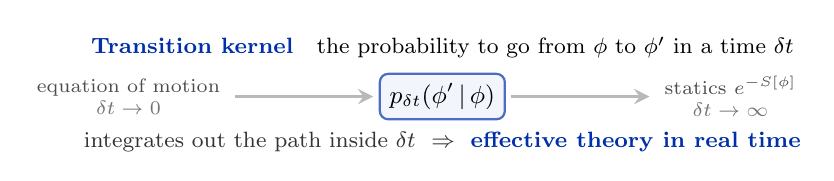
\begin{tikzpicture}[x=1mm, y=1mm, lab/.style={font=\scriptsize, align=center, text=black!70}]
    \node[thread=cA, font=\small] (p) at (0,0) {$p_{\delta t}(\phi'\,|\,\phi)$};
    \node[lab, anchor=east] (eom) at (-27,0) {equation of motion\\ {\color{black!55}$\delta t\to0$}};
    \node[lab, anchor=west] (st) at (27,0) {statics $e^{-S[\phi]}$\\ {\color{black!55}$\delta t\to\infty$}};
    \draw[tlarrow] (eom) -- (p);
    \draw[tlarrow] (p) -- (st);
    \node[font=\footnotesize, anchor=south] at ([yshift=0.6mm]p.north) {\kb{Transition kernel}\quad the probability to go from $\phi$ to $\phi'$ in a time $\delta t$};
    \node[font=\footnotesize, text=black!80, anchor=north, inner sep=0.5pt] at ([yshift=-1.2mm]p.south) {integrates out the path inside $\delta t$ \ $\Rightarrow$ \ \kb{effective theory in real time}};
  \end{tikzpicture}\par
  \venue{\textbf{Tan}, Li, Wang, arXiv:2610.00546}
\end{frame}

% ---------------------------------------------------------------- 12
\begin{frame}{The effective theory predicts long-time scaling laws}
  \centering
  {\small 2D Model B, conserved dynamics from alloys to the QCD critical point\\[0.15em]
  $\partial_t\phi=\Gamma\nabla^2\,\delta S/\delta\phi+\zeta$ makes the pairs, the network never sees it\par}
  % one picture, so headings, plots and captions of the two results share rows
  \begin{tikzpicture}[x=1mm, y=1mm, res/.style={font=\small, align=center, anchor=north}]
    \node[font=\bfseries, text=Kleinblue] at (25,0) {Critical slowing down};
    \node[font=\bfseries, text=Kleinblue] at (80,0) {Coarsening};
    \node[inner sep=0pt] at (25,-16.5) {\includegraphics[height=2.6cm]{collapse_dm_L32}};
    % panel (a) of collapse_dm_L128.pdf, colour bar and lower panel cut away
    \node[inner sep=0pt] at (80,-16.5) {\includegraphics[width=5.2cm, trim=36bp 192.2bp 0 0, clip]{collapse_dm_L128.pdf}};
    \node[res] at (25,-31) {$\tau\propto k^{-z}$, learned $z=3.79(2)$\\ direct simulation $3.81(2)$};
    \node[res] at (80,-31) {domain size $\propto t^{1/3}$\\ train $L\le64$, generate $L=128$};
  \end{tikzpicture}\par
  \vspace{-0.2em}
  {\small\kb{train at $t=0$--$10$, predict $t=0$--$2000$}\par}
  {\small neither law is in the pairs, both emerge at $t\gg\delta t$\par}
  {\kb{Faster than any public SOTA SPDE solver}\par}
  \venue{\textbf{Tan}, Li, Wang, arXiv:2610.00546}
\end{frame}

% ---------------------------------------------------------------- 13
\begin{frame}{Colloids in an optical potential}
  \begin{columns}[T,onlytextwidth]
    \begin{column}{0.44\textwidth}
      \centering
      \vspace{0.2em}
      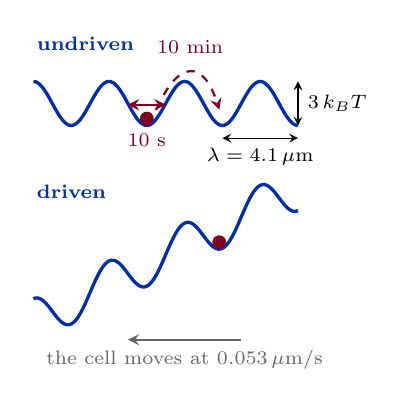
\begin{tikzpicture}[font=\scriptsize, >=stealth, x=1cm, y=1cm, scale=0.8]
        % period 1.2 cm stands for lambda = 4.1 um, minima at x = 0.6 + 1.2 n
        \node[anchor=west, font=\scriptsize\bfseries, text=Kleinblue] at (-0.1,0.95) {undriven};
        \draw[very thick, Kleinblue, domain=0:4.2, samples=120, smooth] plot (\x,{0.35*cos(deg(2*pi*\x/1.2))});
        \fill[burgundy] (1.8,-0.24) circle (0.11);
        % the 10 s label sits under the particle, inside the well it would cross the curve
        \draw[<->, burgundy, thick] (1.5,-0.02) -- (2.1,-0.02);
        \node[text=burgundy] at (1.8,-0.58) {$10$ s};
        \draw[->, burgundy, thick, dashed] (1.95,-0.1) .. controls (2.3,0.7) and (2.7,0.7) .. (2.95,-0.1) node[midway, above=3pt] {$10$ min};
        \draw[<->] (3.0,-0.55) -- (4.2,-0.55) node[midway, below] {$\lambda=4.1\,\mu$m};
        \draw[<->] (4.2,-0.35) -- (4.2,0.35) node[midway, right] {$3\,k_BT$};
        % in the camera frame the moving cell drags the fluid, a constant force, so the washboard tilts
        \begin{scope}[yshift=-2.4cm]
          \node[anchor=west, font=\scriptsize\bfseries, text=Kleinblue] at (-0.1,1.0) {driven};
          \draw[very thick, Kleinblue, domain=0:4.2, samples=160, smooth] plot (\x,{0.35*cos(deg(2*pi*\x/1.2))+0.5*\x-1.05});
          \fill[burgundy] (2.95,{0.35*cos(deg(2*pi*2.95/1.2))+0.5*2.95-1.05+0.11}) circle (0.11);
          \draw[->, thick, black!60] (3.3,-1.35) -- (1.5,-1.35) node[midway, below] {the cell moves at $0.053\,\mu$m/s};
        \end{scope}
      \end{tikzpicture}\\[0.3em]
      \includegraphics[height=1.5cm]{colloid_tracks.png}
    \end{column}
    \begin{column}{0.54\textwidth}
      \small\raggedright
      \kb{The experiment}\\
      about $1200$ colloids, tracked for\\ $60$ min undriven, $30$ min driven\\[0.5em]
      \kb{Two time scales}\\
      in a well $\sim10$ s, escape $\sim10$ min\\
      moving the cell tilts the washboard\\[0.5em]
      \kb{Given}\\
      pairs $(x_t,x_{t+\delta t})$, $\delta t=10$ s\\
      from the first $10$ min only\\
      no potential, drive or noise model
    \end{column}
  \end{columns}
  \venue{\textbf{Tan}, Li, Wang, arXiv:2610.00546}
  \refs{%
    \rtag{Experiment} Dieball et al., Soft Matter 21, 2170 (2025).\quad
    \rtag{Kernel} conditioned on the position within one period.}
\end{frame}

% ---------------------------------------------------------------- 14
\begin{frame}{Ten minutes of data predict the next twenty}
  \begin{columns}[T,onlytextwidth]
    \begin{column}{0.49\textwidth}
      \centering
      \kb{Driven}\\[0.1em]
      % panel (e) of experiment_endmatter.pdf
      \includegraphics[width=0.58\linewidth, trim=0 0 383.4bp 113.4bp, clip]{experiment_endmatter.pdf}
    \end{column}
    \begin{column}{0.49\textwidth}
      \centering
      \kb{Undriven}\\[0.1em]
      % panel (a) of experiment_endmatter.pdf
      \includegraphics[width=0.58\linewidth, trim=0 117bp 383.4bp 0, clip]{experiment_endmatter.pdf}
    \end{column}
  \end{columns}
  \vspace{0.2em}
  {\centering\scriptsize
  \tikz[baseline=-0.6ex]\draw[black!80, line width=0.6pt] (0,0) circle (0.7mm); data\quad
  \tikz[baseline=-0.6ex]\draw[dmline, line width=1.2pt] (0,0) -- (4mm,0); learned kernel\quad
  \tikz[baseline=-0.6ex]\draw[lvline, dashed, line width=1.2pt] (0,0) -- (4mm,0); Langevin\quad
  \tikz[baseline=-0.6ex]\draw[black!60, dotted, line width=0.8pt] (0,-1.2mm) -- (0,1.2mm); end of training\par}
  \vspace{0.5em}
  {\centering\footnotesize
  \renewcommand{\arraystretch}{1.15}
  \begin{tabular}{@{}l@{\hspace{1.6em}}c@{\hspace{1.6em}}c@{\hspace{1.6em}}c@{}}
    & data & \textcolor{dmline}{learned kernel} & \textcolor{lvline}{Langevin}\\
    \midrule
    driven mean velocity [$\mu$m/s] & $-0.0282(3)$ & \textcolor{dmline}{$-0.0284$} & \textcolor{lvline}{$-0.0298$}\\
    driven passage time [s] & $168(4)$ & \textcolor{dmline}{$166.5$} & \textcolor{lvline}{$157.3$}\\
    undriven drift [$\mu$m/s] & $0.0005(1)$ & \textcolor{dmline}{$0.0006$} & \textcolor{lvline}{$0$}\\
    \bottomrule
  \end{tabular}\par}
  \venue{\textbf{Tan}, Li, Wang, arXiv:2610.00546}
  \refs{%
    \rtag{Langevin model} Dieball et al., Soft Matter 21, 2170 (2025).\quad
    Passage time, the first arrival one period downstream. Means over the predicted window.}
\end{frame}

\section{Research plan}

% ---------------------------------------------------------------- 15
\begin{frame}{My research plan in the AI as Science team}
  \centering
  \vspace{0.8em}
  {\large\kb{Extend the current work,\\ and build the RG into AI}\par}
  \vspace{1.6em}
  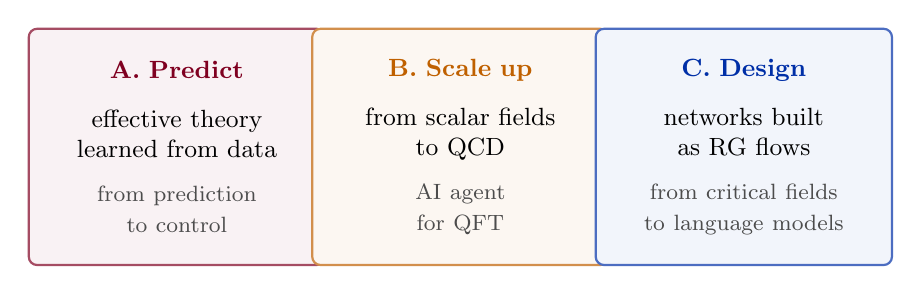
\begin{tikzpicture}[x=1mm, y=1mm]
    \foreach \x/\col/\head/\body/\foot in {
        0/cB/{A.\ Predict}/{effective theory\\ learned from data}/{from prediction\\ to control},
        36/cC/{B.\ Scale up}/{from scalar fields\\ to QCD}/{AI agent\\ for QFT},
        72/cA/{C.\ Design}/{networks built\\ as RG flows}/{from critical fields\\ to language models}}
      \node[thread=\col, align=center, anchor=north, text width=0.29\textwidth, minimum height=30mm, font=\small] at (\x,0)
        {{\bfseries\color{\col}\head}\\[0.7em] \body\\[0.7em] {\footnotesize\color{black!70}\foot}};
  \end{tikzpicture}\par
  \vspace{1.4em}
  {\small AI research grounded in field theory, for the natural and social sciences\par}
\end{frame}

% ---------------------------------------------------------------- 16
\begin{frame}{Extending the current work}
  \vspace{0.1em}
  % one picture for the whole page, so every row sits at a fixed height
  \begin{tikzpicture}[x=1mm, y=1mm,
      lab/.style={font=\scriptsize, anchor=north, align=center},
      team/.style={font=\tiny, text=black!60, anchor=north, align=center}]
    \node[anchor=west, inner sep=0pt] at (0,0) {{\color{cB}\bfseries A.\ Predict}\quad{\small effective theory learned from short-time observations}};
    \node[anchor=south, inner sep=0pt] at (13.5,-16) {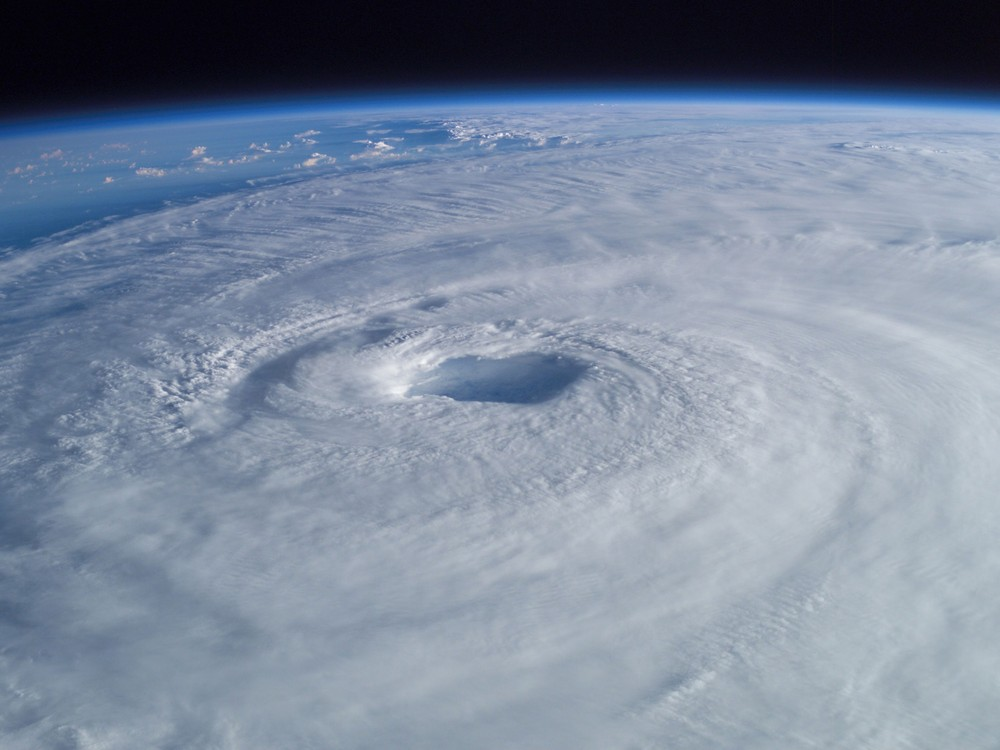
\includegraphics[height=1.1cm]{hurricane_isabel.jpg}};
    \node[anchor=south, inner sep=0pt] at (40.5,-16) {\includegraphics[height=1.1cm]{myoglobin.png}};
    % a flock, every bird a small triangle with nearly the same heading
    \begin{scope}[shift={(62,-16)}, x=0.55mm, y=0.55mm]
      \draw[black!15] (0,0) rectangle (20,20);
      \foreach \x/\y/\a in {3/4/30, 7/3/25, 11/5/35, 15/4/28, 4/9/22, 9/10/33, 13/9/27, 17/11/31,
                            3/15/26, 8/16/29, 12/14/36, 16/17/24, 6/12/32, 10/6/21, 14/13/30}
        \fill[cB!80, rotate around={\a:(\x,\y)}] (\x+1.2,\y) -- (\x-0.8,\y+0.7) -- (\x-0.4,\y) -- (\x-0.8,\y-0.7) -- cycle;
    \end{scope}
    \node[anchor=south, inner sep=0pt] at (94.5,-16) {\includegraphics[height=1.1cm]{colloid_tracks.png}};
    \foreach \x/\name/\team in {13.5/weather/{Prediction Science}, 40.5/{protein motion}/{iTHEMS biology}, 67.5/{collective behavior}/{Mathematical\\ Social Science}} {
      \node[lab] at (\x,-16.8) {\name};
      \node[team] at (\x,-20) {\team};
    }
    \node[lab] at (94.5,-16.8) {colloid experiment};
    \node[team] at (94.5,-20) {active/soft matter\\ \textcolor{cA}{done}};

    \node[anchor=west, inner sep=0pt] at (0,-30) {{\color{cC}\bfseries B.\ Scale up}\quad{\small one sampler across volume, coupling and lattice spacing}};
    \foreach \x/\name/\st [count=\i] in {15/{scalar $\phi^4$}/done, 41/{gauge fields}/{started, SU(3)}, 67/{fermions}/{started, Yukawa}, 93/{QCD}/goal} {
      \node[thread=cC, align=center, text width=19mm, minimum height=6.5mm, font=\small] (s\i) at (\x,-38) {\name};
      \node[font=\scriptsize, text=black!60, anchor=north] at (\x,-41.8) {\st};
    }
    \draw[tlarrow] (s1) -- (s2); \draw[tlarrow] (s2) -- (s3); \draw[tlarrow] (s3) -- (s4);
    % Aim 4 of the proposal, widened to lattice and pQCD. The agent derives and codes in parallel, physics tests both, and a failed test goes back into the prompt or plan
    \node[font=\footnotesize] at (54,-49.4) {{\bfseries\color{cC}AI agent for QFT}\quad faster fRG, lattice and pQCD research};
    \foreach \x/\n/\head/\txt in {15.25/plan/Plan/{a prompt becomes\\ a list of steps}, 92.75/check/Check/{known observables\\ and symmetries}}
      \node[thread=cC, align=center, text width=25.5mm, minimum height=14.6mm, font=\footnotesize] (\n) at (\x,-59.8) {{\bfseries\color{cC}\head}\\ \txt};
    % two boxes of 6.5mm with a 1.6mm gap span the 14.6mm of Plan and Check
    \foreach \y/\n/\head/\txt in {-55.75/derive/Derive/{tedious derivations}, -63.85/code/Code/{lattice field theory}} {
      \node[thread=cC, text width=37mm, minimum height=6.5mm, font=\footnotesize] (\n) at (54,\y) {\makebox[10.5mm][l]{\bfseries\color{cC}\head}\txt};
      \draw[tlarrow] (plan.east |- \n) -- (\n.west);
      \draw[tlarrow] (\n.east) -- (check.west |- \n);
    }
    \draw[->, >=stealth, line width=1pt, gray!60, rounded corners=3pt] (check.south) -- ++(0,-2.5) -| (plan.south);
    \node[font=\scriptsize, text=black!60, anchor=north] at (54,-70.3) {revise the prompt or plan};
  \end{tikzpicture}
\end{frame}

% ---------------------------------------------------------------- 17
\begin{frame}{C. RG-inspired network architecture}
  \centering
  \vfill
  % the RG fixes only the layout, so the page claims no exact RG
  \kb{Borrow the structure of the RG}\par
  \vspace{1.2em}
  % each row reads left to right, an RG idea and the design choice it suggests. RG in burgundy, the QFT colour of page 1, the network in blue, its ML colour.
  % RG icons are centred at x=9, network icons at x=65, rows at y=0, -16, -32
  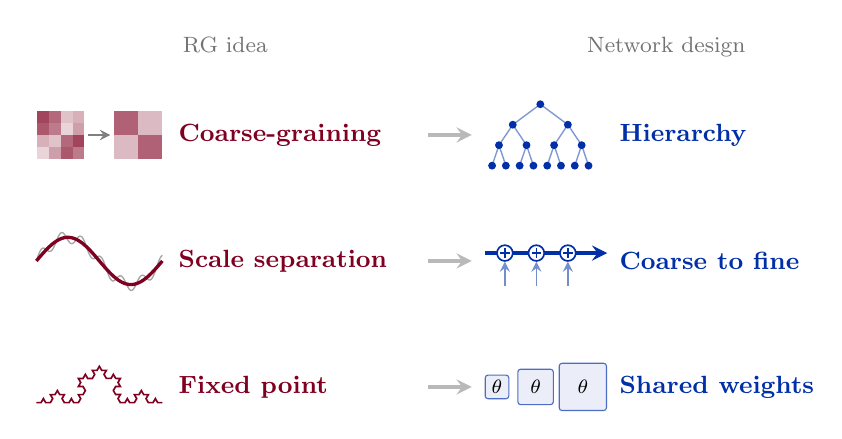
\begin{tikzpicture}[x=1mm, y=1mm, >=stealth,
      txt/.style={anchor=west, inner sep=0pt, font=\small\bfseries},
      head/.style={anchor=base, font=\footnotesize, text=black!55}]
    \node[head] at (25,10.5) {RG idea};
    \node[head] at (81,10.5) {Network design};
    \foreach \y in {0,-16,-32} \draw[tlarrow] (50,\y) -- (57,\y);
    \node[txt, text=cB] at (19,0) {Coarse-graining};
    \node[txt, text=cB] at (19,-16) {Scale separation};
    \node[txt, text=cB] at (19,-32) {Fixed point};
    \node[txt, text=cA] at (75,0) {Hierarchy};
    \node[txt, text=cA] at (75,-16) {Coarse to fine};
    \node[txt, text=cA] at (75,-32) {Shared weights};
    % block spin, 4x4 sites averaged to 2x2. Shades are 10+70v for site values v
    \begin{scope}[shift={(1.1,3)}]
      \foreach \c [count=\k from 0] in {73,59,24,31,66,52,17,38,31,24,59,73,17,38,66,52} {
        \pgfmathtruncatemacro\cx{mod(\k,4)}
        \pgfmathtruncatemacro\cy{div(\k,4)}
        \fill[cB!\c] (1.5*\cx,-1.5*\cy) rectangle ++(1.5,-1.5);
      }
      \draw[->, black!50, line width=0.7pt] (6.5,-3) -- (9.3,-3);
      \foreach \c [count=\k from 0] in {62,27,27,62} {
        \pgfmathtruncatemacro\cx{mod(\k,2)}
        \pgfmathtruncatemacro\cy{div(\k,2)}
        \fill[cB!\c] (9.8+3*\cx,-3*\cy) rectangle ++(3,-3);
      }
    \end{scope}
    % a field and its long-wavelength part, the wiggles are what coarse-graining drops
    \begin{scope}[shift={(1,-16)}]
      \draw[black!35, line width=0.5pt, domain=0:16, samples=160, smooth] plot (\x,{3*sin(deg(2*pi*\x/16))+0.75*sin(deg(2*pi*6.3*\x/16))});
      \draw[cB, line width=1.2pt, domain=0:16, samples=60, smooth] plot (\x,{3*sin(deg(2*pi*\x/16))});
    \end{scope}
    % Koch curve, the same shape at every magnification
    \draw[cB, line width=0.6pt] decorate[decoration=Koch snowflake] {decorate[decoration=Koch snowflake] {decorate[decoration=Koch snowflake] {(1,-34) -- (17,-34)}}};
    % binary tree, each level halves the number of sites
    \begin{scope}[shift={(65,-3.9)}]
      \foreach \l in {0,1,2} {
        \pgfmathtruncatemacro\n{2^(3-\l)}
        \foreach \i in {1,...,\n} {
          \pgfmathsetmacro\xa{(\i-0.5)*14/\n-7}
          \pgfmathtruncatemacro\p{ceil(\i/2)}
          \pgfmathsetmacro\xb{(\p-0.5)*28/\n-7}
          \draw[cA!50, line width=0.5pt] (\xa,2.6*\l) -- (\xb,2.6*\l+2.6);
        }
      }
      \foreach \l in {0,1,2,3} {
        \pgfmathtruncatemacro\n{2^(3-\l)}
        \foreach \i in {1,...,\n} {
          \pgfmathsetmacro\xa{(\i-0.5)*14/\n-7}
          \fill[cA] (\xa,2.6*\l) circle (0.5);
        }
      }
    \end{scope}
    % the coarse field runs straight through, each level only adds its details
    \begin{scope}[shift={(65,-15)}]
      \draw[->, cA, line width=1.4pt] (-7,0) -- (8.5,0);
      \foreach \x in {-4.5,-0.5,3.5} {
        \draw[->, cA!55, line width=0.6pt] (\x,-4.2) -- (\x,-1.1);
        \draw[cA, line width=0.6pt, fill=white] (\x,0) circle (1);
        \draw[cA, line width=0.6pt] (\x-0.6,0) -- (\x+0.6,0) (\x,-0.6) -- (\x,0.6);
      }
    \end{scope}
    % one set of weights, applied at every scale
    \begin{scope}[shift={(65,-32)}]
      \foreach \s/\x in {3/-5.5, 4.5/-0.6, 6/5.4}
        \node[draw=cA!70, fill=cA!8, rounded corners=1pt, minimum size=\s mm, inner sep=0pt, font=\scriptsize] at (\x,0) {$\theta$};
    \end{scope}
  \end{tikzpicture}\par
  \vfill
\end{frame}

% ---------------------------------------------------------------- 18
\begin{frame}{C. From critical fields to language models}
  \centering
  \vspace{0.2em}
  \kb{Natural data has scaling}\par
  \vspace{0.6em}
  \begin{columns}[T,onlytextwidth]
    \begin{column}{0.24\textwidth}
      \centering
      \parbox[c][1.45cm][c]{\linewidth}{\centering\includegraphics[height=1.3cm]{phi4_snapshot_k0.2705.png}}\\[0.3em]
      {\small critical field\par}
      {\footnotesize $G(r)\sim r^{-1/4}$\par}
    \end{column}
    \begin{column}{0.24\textwidth}
      \centering
      % a drawn photo icon stands for any image data set
      \parbox[c][1.45cm][c]{\linewidth}{\centering
      
\begin{tikzpicture}[x=1.3mm, y=1.3mm]
        \draw[black!60, line width=0.8pt, rounded corners=1pt] (0,0) rectangle (13,10);
        \fill[black!25] (1,1) -- (4.8,6) -- (7.5,3.2) -- (9.7,5.5) -- (12,1) -- cycle;
        \fill[orange!70] (10,7.8) circle (1.1);
      \end{tikzpicture}}\\[0.3em]
      {\small images\par}
      {\footnotesize $P(k)\sim k^{-2}$\par}
    \end{column}
    \begin{column}{0.24\textwidth}
      \centering
      \parbox[c][1.45cm][c]{\linewidth}{\centering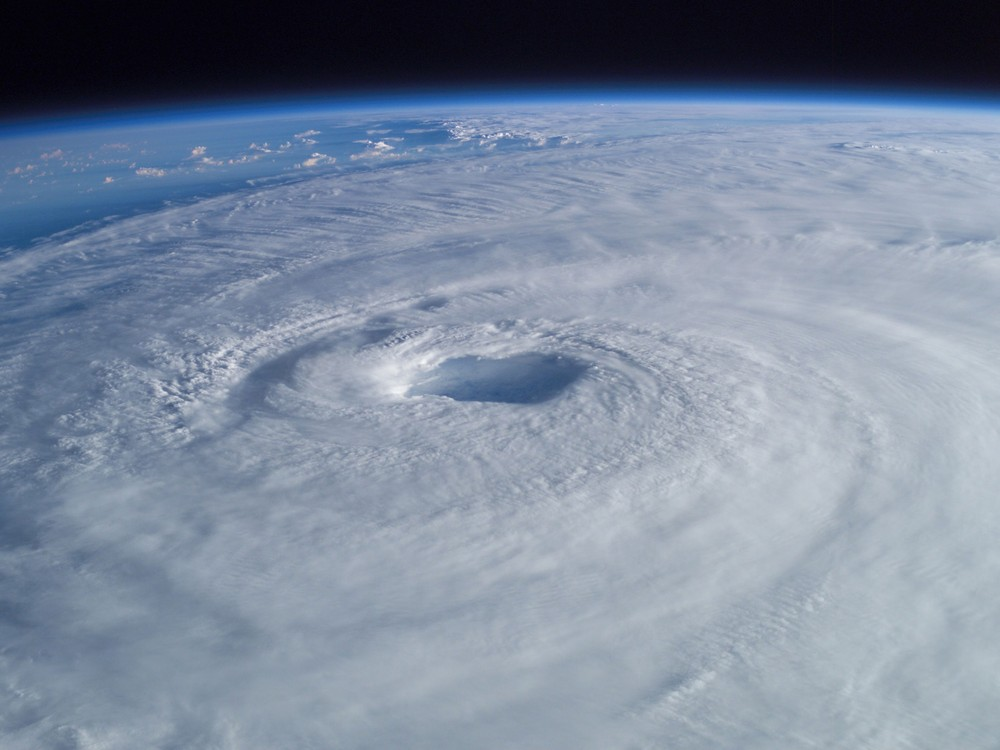
\includegraphics[height=1.3cm]{hurricane_isabel.jpg}}\\[0.3em]
      {\small atmosphere\par}
      {\footnotesize $E(k)\sim k^{-5/3}$\par}
    \end{column}
    \begin{column}{0.24\textwidth}
      \centering
      % words merged pairwise into phrases and a sentence, the block-spin picture of grammar
      \parbox[c][1.45cm][c]{\linewidth}{\centering
      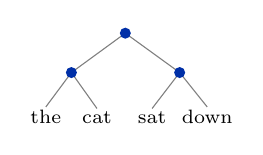
\begin{tikzpicture}[x=1mm, y=1mm]
        \foreach \x/\w [count=\i] in {0/the, 6.5/cat, 13.5/sat, 20.5/down} \node[font=\scriptsize, inner sep=1pt, anchor=base] (w\i) at (\x,0) {\w};
        \coordinate (p1) at (3.25,6.5); \coordinate (p2) at (17,6.5); \coordinate (r) at (10.1,11.5);
        \draw[black!50] (w1.north) -- (p1) -- (w2.north); \draw[black!50] (w3.north) -- (p2) -- (w4.north);
        \draw[black!50] (p1) -- (r) -- (p2);
        \foreach \c in {p1, p2, r} \fill[cA] (\c) circle (0.7);
      \end{tikzpicture}}\\[0.3em]
      {\small language\par}
      {\footnotesize $I(r)\sim r^{-\beta}$\par}
    \end{column}
  \end{columns}
  \vspace{1.6em}
  \kb{What an RG network could change}\par
  \vspace{0.6em}
  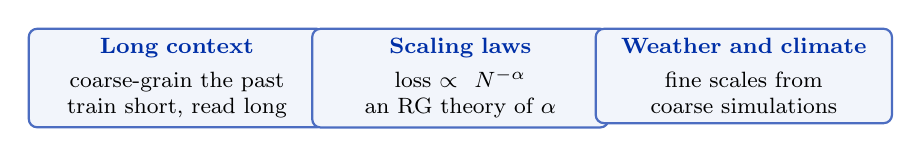
\begin{tikzpicture}[x=1mm, y=1mm]
    \foreach \x/\head/\body in {
        0/{Long context}/{coarse-grain the past\\ train short, read long},
        36/{Scaling laws}/{loss $\propto N^{-\alpha}$\\ an RG theory of $\alpha$},
        72/{Weather and climate}/{fine scales from\\ coarse simulations}}
      \node[thread=cA, align=center, anchor=north, text width=0.29\textwidth, font=\footnotesize] at (\x,0)
        {{\bfseries\color{cA}\head}\\[0.3em] \body};
  \end{tikzpicture}\par
  \refs{Lin, Tegmark, Entropy 19, 299 (2017).\quad Kaplan \textit{et al.}, arXiv:2001.08361.}
\end{frame}

% ---------------------------------------------------------------- Three-year plan, commented out
% \begin{frame}{Three-year plan}
%   \centering
%   \vspace{0.6em}
%   \begin{tikzpicture}[x=1mm, y=1mm]
%     \foreach \c/\yr in {0/Year 1, 1/Year 2, 2/Year 3} \node[font=\small\bfseries, text=black!75] at (24+30*\c, 0) {\yr};
%     \foreach \r/\col/\lab/\a/\b/\c in {
%         0/cB/A/{critical dynamics\\ in real time}/{pilot with\\ an iTHEMS team}/{toward\\ control},
%         1/cC/B/{gauge fields,\\ agent prototype}/{fermions,\\ agent end to end}/{QCD on small\\ lattices},
%         2/cA/C/{RG networks for\\ field theories}/{RG networks for\\ natural images}/{toward language\\ models}} {
%       \node[font=\large\bfseries, text=\col] at (0,-11-16*\r) {\lab};
%       \foreach \x/\txt in {24/\a, 54/\b, 84/\c}
%         \node[thread=\col, align=center, text width=25mm, minimum height=11mm, font=\footnotesize] at (\x,-11-16*\r) {\txt};
%     }
%   \end{tikzpicture}\par
%   \vspace{1.2em}
%   {\small\kb{Deliverables} papers in ML venues and physics journals\\ open data and code, a study group at iTHEMS\par}
% \end{frame}

% ---------------------------------------------------------------- 19
\begin{frame}{Research Support, Collaborations \& Academic Service}
  \centering
  % two grey cards side by side over one full-width card, thin rules between items
  % fQCDLogoFR.png from fqcd-collaboration.github.io/assets/img, dm_qft_logo.png from ModelB/Slides/logo
  \begin{tikzpicture}[x=1mm, y=1mm,
      card/.style={rectangle, rounded corners=4pt, fill=black!4, inner sep=2.5mm, anchor=north west},
      icon/.style={baseline=0.2mm, x=1mm, y=1mm, line width=0.5pt, Kleinblue}]
    \node[card] (sup) at (0,0) {\begin{minipage}[t][48mm][t]{64mm}\raggedright
      {\small\bfseries\color{Kleinblue}\tikz[icon]{\draw (1.8,2.3) circle (1.1); \draw (1.1,1.4) -- (0.7,-0.2) -- (1.5,0.3) (2.5,1.4) -- (2.9,-0.2) -- (2.1,0.3);}\hspace{0.5em}Research Support\par}
      \vspace{1.8mm}
      {\footnotesize Recommendation Program for Young Researchers and Woman Researchers\par}
      {\scriptsize\color{black!55}Miyabi-G, University of Tokyo\par Competitive allocation\par October 2026--March 2027\par}
      \vspace{1.4mm}{\color{black!15}\hrule height 0.4pt}\vspace{1.4mm}
      {\footnotesize\href{https://jhpcn-kyoten.itc.u-tokyo.ac.jp/abstract/EX26314}{JHPCN exploratory joint research}\hfill{\tiny\color{black!55}EX26314}\par}
      {\scriptsize\color{black!55}\jafont 生成モデルを用いた臨界現象のデータ駆動型研究\par}
      \vspace{1.4mm}{\color{black!15}\hrule height 0.4pt}\vspace{1.4mm}
      {\footnotesize Google DeepMind AI for Science\hfill{\tiny\color{black!55}Japan/APAC}\par}
      {\scriptsize\color{black!55}RIKEN iTHEMS--Google DeepMind collaboration on AI-assisted research in quantum field theory\par}
    \end{minipage}};
    \node[card] (col) at (72,0) {\begin{minipage}[t][48mm][t]{29mm}\centering
      {\small\bfseries\color{Kleinblue}\tikz[icon]{\draw (0.9,2.4) circle (0.7) (3.1,2.4) circle (0.7) (-0.1,0) arc[start angle=180, end angle=0, radius=1.0] (2.1,0) arc[start angle=180, end angle=0, radius=1.0];}\hspace{0.5em}Collaborations\par}
      \vspace{2mm}
      \href{https://fqcd-collaboration.github.io/}{\includegraphics[height=7.5mm]{fQCDLogoFR.png}}\par\vspace{0.6mm}
      {\footnotesize fQCD\par}
      {\tiny\color{black!55}fqcd-collaboration.github.io\par}
      % \vfill outranks the \vss of the fixed-height minipage, so the spare height goes around the rule
      \vfill{\color{black!15}\hrule height 0.4pt}\vfill
      \href{https://dm-qft.github.io/homepage/}{\includegraphics[height=8.5mm]{dm_qft_logo.png}}\par\vspace{0.6mm}
      {\footnotesize DM-QFT\par}
      {\tiny\color{black!55}dm-qft.github.io/homepage\par}
    \end{minipage}};
    % heading beside the list, not above it, so three entries stay clear of the frame number
    \node[card] at ([yshift=-3mm]sup.south west) {\begin{minipage}[t]{101mm}
      {\small\bfseries\color{Kleinblue}\tikz[icon]{\draw[rounded corners=0.3mm] (0.3,0) rectangle (3.1,3.6); \draw (0.9,2.7) -- (2.5,2.7) (0.9,1.8) -- (2.5,1.8) (0.9,0.9) -- (2.0,0.9);}\hspace{0.5em}\parbox[t]{17mm}{Academic\\Service}}\hfill
      \parbox[t]{76mm}{\footnotesize Referee · Physical Review D · APS Open Science\\
        Co-organizer · \href{https://sites.google.com/view/deep-in-wg/events/2026-ai4science-summer-school}{AI for Science Summer School}\\
        Member · iTHEMS DEEP-IN Working Group}
    \end{minipage}};
  \end{tikzpicture}\par
\end{frame}

% ---------------------------------------------------------------- 20
\begin{frame}{Summary}
  \centering
  \vspace{2.5em}
  % the three parts of the talk above the three directions of the plan, done in grey, next in the colours of the plan page
  % the strut gives every box the depth of the g in agent, so the boxes of a row end level
  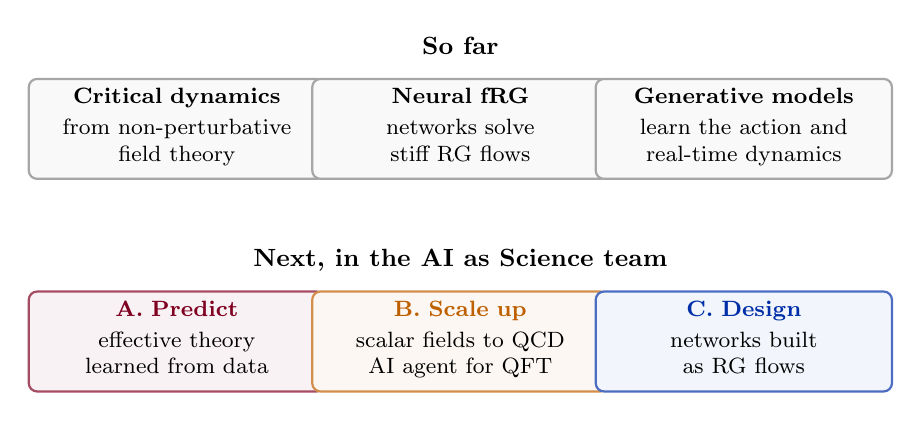
\begin{tikzpicture}[x=1mm, y=1mm,
      row/.style={font=\small\bfseries, anchor=base},
      box/.style={align=center, anchor=north, text width=0.29\textwidth, font=\footnotesize}]
    \node[row] at (52,0) {So far};
    \foreach \x/\head/\body in {
        16/{Critical dynamics}/{from non-perturbative\\ field theory},
        52/{Neural fRG}/{networks solve\\ stiff RG flows},
        88/{Generative models}/{learn the action and\\ real-time dynamics}}
      \node[thread=gray, box] at (\x,-3) {{\bfseries\head}\\[0.2em] \body\strut};
    \node[row] at (52,-27) {Next, in the AI as Science team};
    \foreach \x/\col/\head/\body in {
        16/cB/{A.\ Predict}/{effective theory\\ learned from data},
        52/cC/{B.\ Scale up}/{scalar fields to QCD\\ AI agent for QFT},
        88/cA/{C.\ Design}/{networks built\\ as RG flows}}
      \node[thread=\col, box] at (\x,-30) {{\bfseries\color{\col}\head}\\[0.2em] \body\strut};
  \end{tikzpicture}\par
  % pinned near the bottom edge as in the other talks, so it does not move with the content above
  \begin{tikzpicture}[remember picture, overlay]
    \node[anchor=south, font=\large] at ([yshift=0.45cm]current page.south) {Thank you};
  \end{tikzpicture}
\end{frame}

\end{document}
